% !TeX root = ../main.tex
% Add the above to each chapter to make compiling the PDF easier in some editors.

\chapter{Design \& Implementation}\label{chapter:design}

The goal of this work is to design a system that will allow the verification of closed peer reviews without a trusted third party. The new artifact should improve upon the existing ones, which are the current peer review showcase platforms. Based on the problems identified, the requirements of such a system is defined in the following section. Taking these requirements and available technologies into account, a design of a system will be communicated. Additionally, the implemented proof of concept prototype will be demonstrated.

\section{Requirements} \label{sec:requirements}

As stated in the problem statement, current lack of recognition of peer reviews stems from the public unavailability of the closed peer reviews. Each individual party presented with the peer reviews of a researcher needs to explicitly contact each journal if they want to verify the peer reviews. This is clearly infeasible in a public setting: if a researcher has their peer reviews stated in a public profile, e.g. on their website, each party consuming this data has to contact the journals. This is not the case for other scholarly works such as manuscripts. Therefore, it should be easy to check if the peer review is authentic, that is, the peer reviews are \textbf{verifiable}.

Currently, there are platforms for aggregating and showcasing peer reviews. The process of adding peer reviews to these platforms include automatic methods such as integrations with journals. Users can also add reviews manually such as by sending the review receipt emails or by filling out the review information on the platform. These will get checked by the platform and then the peer review will be "verified". However, it is not possible to trace how the review is verified and it is at the platforms discretion to decide what constitutes a verified review and what is not. There are researchers on these platforms that have over 1000 verified reviews per year on their profile. Questions about the validity of this data has been raised \parencite{TeixeiradaSilva.2020, TeixeiradaSilva.2017, TeixeiradaSilva.2019}. Following the open science principles it is important to provide provenance on data and \textbf{transparency} on how the verification is done.

It is outlined in previous sections, how the review showcasing platforms aggregate review data by acting as trusted third-parties. They become the sources of peer review contributions of a researcher and decide what is a "verified" review. The data stored by the platforms is different than what is available to public, which enables potentially putting the data behind a paywall or charging its users. Therefore, \textbf{open data} is another requirement of the system. In parallel, by having a system design based on \textbf{open standards}, vendor lock-in can be avoided. This lets anybody provide review showcasing services and users will have the freedom to choose which service they want to use. Also, the platforms' ability to hold onto the peer review data is provided by their position as the trusted third-parties.  Instead, it is desirable to create direct trust between the parties. The designed system should facilitate \textbf{direct trust} between the stakeholders. 

A peer review has various metadata associated. The necessary data to be presented may be different in each context. For a review author it is useful to be able present different data associated with the review without breaking the verifiability of the review. For instance, the contents and the date of a closed review may not be shared on a public profile, but a review author might want to share these in a more private setting such as in a job or grant application. In both cases, the reviewer should be able to \textbf{selectively disclose} which attributes they want to share.

Peer review practices vary a lot between fields, even from journal to journal within the same field. Hence, the required system should be \textbf{compatible} with the different practices and different data resulting from these processes. The system should enable the creation of different data schemas, but at the same time avoid ambiguity and let stakeholders communicate what this data means.

Here the requirements are listed together once again.
\begin{itemize}
  \item RQ1: Verifiability \label{rq:verifiable}
  \item RQ2: Transparency \label{rq:transparent}
  \item RQ3: Open Data \label{rq:open-data}
  \item RQ4: Open Standards \label{rq:open-standards}
  \item RQ5: Direct Trust \label{rq:direct-trust}
  \item RQ6: Selective Disclosure \label{rq:selective-disclosure}
  \item RQ7: Compatibility \label{rq:compatible}
\end{itemize}

\section{Design}

%% TODO: Why I choose JSON-LD over JWT see https://www.w3.org/TR/vc-imp-guide and Kaliya Young's doc
% "The relying party (verifier) is left guessing about the meaning, and if they don’t want to guess, they must find an out-of-band way to connect back to the issuer to figure out the meaning."

% Why is the review the subject
% Because it is "the" credential. We make a Peer Review Credential. A peer review authorship credential is trivial.

% We don't care how the credential is transferred. g DIDComm, pairwise connection using JWT, SIOP CHAPI etc.

\subsection{Overview}

As the basis the W3C's Verifiable Credentials specification \parencite{Sporny.18Kas2019} is chosen. The specification inherently satisfies some of the requirements of the system. It is verifiable \hyperref[rq:verifiable]{(RQ1)}, based on open standards \hyperref[rq:open-standards]{(RQ4)}, and built with an open world assumption, that is, anyone can extend the existing vocabularies and can issue credentials \hyperref[rq:compatible]{(RQ7)}. Also, there exist open source \acrshort{VC} libraries that can be used in the implementation.

The designed system has two main components:

\begin{enumerate}
    \item \textbf{Journal X:} A hypothetical journal that issues peer review credentials
    \item \textbf{Veriview:} An open source peer review showcase platform that supports peer review \acrshort{VC}s
\end{enumerate}


In a typical peer review process, a researcher receives an invitation to do a peer review from the editor of the journal. Here, upon receiving an invitation from Journal X, the reviewer accepts it and submits the review of the manuscript to Journal X. Then she can request the proof of their work as a peer review verifiable credential. Journal X prepares the credential and issues it by signing the document. The review author can use this credential to prove their authorship. A peer review showcasing platform called Veriview is also conceived, where review authors can build their "peer review resume". According to the privacy policy of the review, they can decide which information about the review to share publicly. For instance, a blinded review typically can not be shared with identifiable information such as the manuscript, the content, the title etc. The reviewer is able to choose which information to share on their public profile accordingly. An overview of the interactions of the typical use case on the system are depicted below in Figure \ref{fig:sequence1} 

\begin{figure}[htpb]
  \centering
  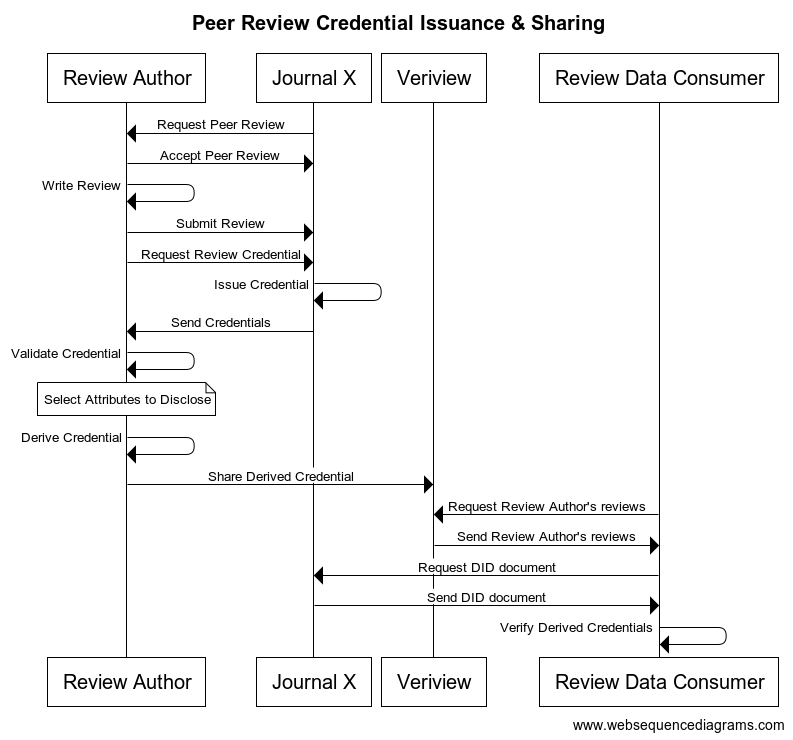
\includegraphics[width=0.8\textwidth]{figures/sequence.png}
  \caption{Overview of peer review credential issuance and sharing process} \label{fig:sequence1}
\end{figure}

In practice, there supposed to be many journals and Journal X is one example out of numerous journals. Also Veriview is not a single platform but there may be many showcasing platforms that researchers can choose to build their profiles at. Having a system based on open standards \hyperref[rq:open-standards]{(RQ4)} allows anyone to create a platform similar to Veriview and this would avoid vendor lock-in. 

Additionally assumed is a "Review Data Consumer", a party which is interested in the peer review data of a reviewer. In real world these might be employers, universities, research institutions, or other researchers. This can also be other applications that want to make use of the peer review contributions of researchers. For example, a peer review matching application that would suggest potential reviewers to editors or platforms aiming to incentivize reviewers \parencite{TenorioFornes.2019, Jan.2018c, TrovoMassari} with rewards can make use of this open data \hyperref[rq:open-data]{(RQ3)}.  Any party that is interested in the peer reviews of a researcher, and their authenticity, might be a consumer. 

The use case depicted in Figure \ref{fig:sequence1} assumes the reviews are shared publicly and are not open reviews. Open reviews would not require additional derivation as all of the review data can be shared publicly and they are verifiable themselves where they are published. Since Veriview is a platform to share blinded peer reviews publicly, the review author will choose which attributes they want to and are able to share, and derive a credential containing the selected attributes and a zero-knowledge proof which can be shared in Veriview. 

In a private setting or for an open review this additional derivation step is not required. For instance, if the researcher wants to include their review in a grant application, they might want to share the reviewed manuscript and the contents of the review. If the manuscript is in the scientific field the researcher wants to show competence in, being able to verifiably show that they were invited and done a review in this field  would demonstrate the researcher's competence. Also, other factors such as the journal's reputation provide additional information. In this case Veriview is not required and the interactions are as in Figure \ref{fig:sequencePrivate}.

\begin{figure}[htpb]
  \centering
  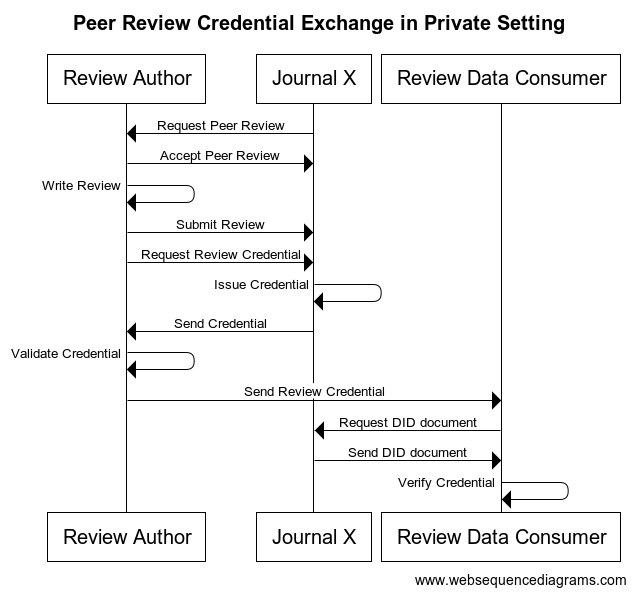
\includegraphics[width=0.8\textwidth]{figures/sequencePrivate.png}
  \caption{Peer review credential exchange in a private setting} \label{fig:sequencePrivate}
\end{figure}

\subsection{Peer Review Credential}

The Peer Review Credential is a document issued by a journal that a peer review has been done for this journal. The document contains the review content and the metadata associated such as the date, title, author etc. An example credential is given below in Listing \ref{lst:exampleReview}

\lstinputlisting[language=json, caption={Example Peer Review Credential},label={lst:exampleReview}]{code/exampleReviewCredential.json}

The credential in this design follows the \acrshort{JSON-LD} syntax. \acrshort{JSON-LD} is the predominantly used format in the \acrshort{VC} specification. It is also an open standard under W3C \parencite{jsonld} \hyperref[rq:open-standards]{(RQ4)} and many of the \acrshort{VC} libraries available are \acrshort{JSON-LD} based.  \acrshort{JSON-LD}s with Linked Proofs supports Zero-Knowledge Proof formats and \acrshort{JSON-LD}s require canonicalization, which allows flexibility in the order of the attributes. This becomes useful for instance when transferring the credential from the journal to the author, the journal doesn't have to worry about the order of the attributes when they issue the credential. Also, being fully compatible with \acrshort{JSON}, the format easily integrates with existing web frameworks. 

The credential is designed to represent the review as the subject. Under \lstinline{credentialSubject} the data related to review is contained, including the \lstinline{author} field which represents the author of the review. An alternative representation could be to issue a "review authorship" credential which would contain the author as the credential subject and an \lstinline{authoredReview} field containing the review data. Both are valid expressions of the same relationships, but here it is chosen to represent the review itself as the system is for "peer review credentials" and a peer review credential implies the review itself is the credential being issued. In the other case, it is needed to express the credential as a "peer review authorship credential" explicitly and this might create confusion.

\subsubsection{Context}

\lstinline{@context} defines the vocabularies used in the document. The first \acrshort{URL} refers to the \acrshort{VC} context and it is required to be included in all verifiable credentials according to the specification. The second context contains the vocabulary specific for peer reviews which is defined for this system. Finally, \lstinline{https://w3id.org/security/bbs/v1} provides the vocabulary for the \lstinline{BbsBlsSignature} signature suite since it is not included in the default \lstinline{https://www.w3.org/2018/credentials/v1} context. The context used in this document is given in Listing \ref{lst:peer-review-context}

\lstinputlisting[language=json, caption={Peer Review Vocabulary},label={lst:peer-review-context}]{code/peerReviewContext.json}

The vocabulary document itself is a context that defines three different contexts, namely \lstinline{PeerReviewCredential}, \lstinline{PeerReview}, and \lstinline{PeerReviewAuthor}. These contexts can be included in the corresponding objects in the credential by adding to the \lstinline{type} field in the \acrshort{JSON-LD} credential document. The \lstinline{@version} term defines the \acrshort{JSON-LD} version of the definition. This will explicitly tell the \acrshort{JSON-LD} processor to use the version 1.1 processing mode. It is not a requirement to set the version explicitly but this practice avoids potentially processing the document with the older \acrshort{JSON-LD} processors. 


In the vocabulary, terms from \url{schema.org} was used when there exist a clearly overlapping term in the schema.org ontology, such as the \acrshort{ISSN} field or the title field which corresponds to \url{schema.org/headline}. In other cases, self-referring definitions are made, which refer to themselves in the \lstinline{@id} field, as in the case with the \lstinline{author} or \lstinline{journal} fields. There exists a term for \lstinline{author} in schema.org but it is preferred for the schema to be explicit and to be included in credential document through adding the \lstinline{PeerReviewAuthor} in the \lstinline{type} field. Similarly, an explicit definition of \lstinline{journal} is preferred over the general \lstinline{schema.org/Periodical} term. Also, by defining the term \lstinline{"schema": "http://schema.org/"} it is made possible to map the \acrshort{URL} paths to the schema.org. As an example, this allows \lstinline{schema:name} to be expanded into \lstinline{http://schema.org/name} when processed. 

The previous version of the defined peer review vocabulary included \lstinline{@protected: true} attributes in \lstinline{@context}'s, which prevents overriding attributes by new definitions. Even though this adds extra protection to term definitions, it disallows the extension on the definitions. It is removed to enable extensibility. The peer review process varies a lot at each publisher or journal, and issuers can adopt the vocabularies according to their needs. The vocabulary assumes a basic credential model with few attributes associated with a peer review. Thanks to the extensibility of \acrshort{JSON-LD} vocabularies, it possible to extend the vocabulary itself, or include other vocabularies in the document. For instance, if the peer review process of a journal has a statistical soundness check, this can be represented as a \lstinline{statisticallySound} field defined in another vocabulary and included in the credential context. This enables the compatibility of the system \hyperref[rq:compatible]{(RQ7)} with different peer review processes.  Ideally, these vocabularies will be defined with different stakeholders of the peer review ecosystem coming together, that they will be widely accepted and used.


\subsubsection{Signatures}

Expressed by the \lstinline{BbsBlsSignatureProof2020} type in the \lstinline{proof} field, BBS+ signatures with a BLS12-381 curve is the chosen signature suite. BBS+ signatures is the preferred signature scheme while BLS12-381 is the curve used for generating the keys. BBS+ signatures can be used with any pairing friendly curve \parencite{irtf-cfrg-pairing-friendly-curves-09}, but since the existing Linked Data Proof signature suite \parencite{looker_steele_2021} and the implementations\footnote{https://github.com/mattrglobal/bbs-signatures-spec} are based on BLS12-381 curves, the same curve was adopted. This signature suite allows zero-knowledge selective disclosure of attributes \hyperref[rq:selective-disclosure]{(RQ6)} with more efficient size and execution times \parencite{anoncreds} compared to the existing ones such as \acrshort{CL} signatures. 

With BBS+ signatures it is possible to sign multiple messages. The signature scheme provides a $sign$ and a $verify$ verify function that are also found in other digital signature schemes. The signature is not over the whole message and the size of the signature is variable with the number of messages hidden. For an array of messages $m[0], m[1], ..., m[n]$, a public key $privk$, a private (secret) key $pubk$ the below functions are provided.

\[signature = sign((m[0], m[1], ..., m[n]), pubk, privk)\]

\[result = verify((m[0], m[1], ..., m[n]), signature, pubk)\]

Where result is a boolean value representing the validity of the signature. Additionally, the BBS+ signatures allows derivation of a \textit{proof} of knowledge of the original signature and the verification of the proof. A party who knows the messages, the public key, and the signature over all of the messages can take a subset of the messages and create a zero-knowledge proof as follows:

\[proof = derive( (m[3], m5],..., m[n-1]), signature, pubk)\]

Which can be verified with: 

\[result = verifyProof( (m[3], m[5],..., m[n-1]), proof, pubk) \]

With the BLS12-381 curve the element sizes are as follows \parencite{mattrglobal_2021}:
\begin{center}
\begin{tabular}{ c c }
  Element & Size    \\
  \hline
  $privk$   &   32 bytes    \\
  $pubk$    &   96 bytes    \\
  $signature$ & 112 bytes   \\
  $proof$   &   368 + (hidden message count) x 32 bytes
\end{tabular}
\end{center}

\subsubsection{Decentralized Identifiers}

The \acrshort{VC} specification describes several attributes as identifiers (i.e. \acrshort{URI}s). Apart from uniquely identifying the described object, these fields may also be used for authentication. In the case of \lstinline{issuer}, the value of the attribute is recommended to resolve to a document that can be used to verify the credential. The document would contain the public key information of the signer key, and other meta-data related to the issuer. Similarly, a \acrshort{DID} in the \lstinline{author} field can be used for verification in a credential exchange. The holder of the credential (author) can wrap the credential or multiple credentials in a verifiable presentation to ensure it is being sent from the intended holder. 

In this system, the issuer field is a \acrshort{DID} of the journal. It is required for the verifiability of the peer reviews to have this identifier field resolve to a document with a public key \hyperref[rq:verifiable]{(RQ1)}. Although it is possible to use an \acrshort{HTTP} \acrshort{URL} that resolve to a document containing public keys, \acrshort{DID}s are preferred since it provides a standard document format that can be used for verification, and for their close relationship with \acrshort{VC}s in the \acrshort{SSI} ecosystem. 

Using a \acrshort{DLT} based \acrshort{DID} method would provide the document a high availability, tamper-proofness, and won't require to contact the issuer at each verification. An example would be \lstinline{did:sov:mnjkl98uipsndg2hdjdjuf7} which represents a DID that can be resolved with the Sovrin blockchain method. However, it would be necessary to bind this \acrshort{DID} with the real world identity of the journal. By looking at the identifier \lstinline{did:sov:mnjkl98uipsndg2hdjdjuf7}, a third-party is not able to infer that this is the identity associated with Journal X. In that case, the identifier \lstinline{did:sov:mnjkl98uipsndg2hdjdjuf7} needs to be announced as belonging to Journal X in different channels. This may be in a non-digital communication or by announcing the identifiers on the journal website. An alternative in the \acrshort{DID} space is to create accreditation registries. Similar to accreditation in real world, a third party or a joint organization can keep a registry of vouched identities, and can provide the necessary trust. However, this may lead to centralization and is similar to the centralization vs. decentralization dichotomy in the web \acrshort{PKI} systems \parencite{Perlman1999}.

Here, \lstinline{did:web}\footnote{https://w3c-ccg.github.io/did-method-web/} is the preferred \acrshort{DID} method used for the \lstinline{issuer} field. Compared to a \acrshort{DLT} method this would require the server of the \acrshort{DID} document to be highly available and the controller of the server may change the file without others noticing. The advantage is that this method makes use of the identity provided by the journal's host address (e.g. https://www.journalx.com) and its X.509 certificate \parencite[4]{Barclay.6Nis2020}. The website of journals are usually known and can serve as a valid identifier thanks to the existing public key infrastructure. It is also human readable, and there exist implementations of \lstinline{did:web} resolvers. To have a \acrshort{DID} document resolved from its identifier, a host can serve it under the well-known path \parencite{rfc5785} \lstinline{https://<HOST-NAME>/.well-known/did.json}. 

Also, as the \lstinline{author} identifier a \acrshort{DID} can be used. The example credential in Listing \ref{lst:exampleReview} contains a \lstinline{did:key} \acrshort{DID} \parencite{did-key} that has its identifier as the Multibase format \parencite{multiformats-multibase-03} of its public key and simply expands to a document containing the same public key used for different verification methods. It is also possible to use different \acrshort{DID}s such as a \acrshort{DLT} based one. By resolving the \acrshort{DID} to a \acrshort{DID} document, the authentication of the holder can be done. In our case, it will enable authenticating that the party presenting the credentials (holder) are actually the author stated in the \lstinline{author} field. This can be done by wrapping the credentials in a verifiable presentation. In theory any identifier field can be a \acrshort{DID} but this comes at the cost and effort of the management of the identity and the keys.

\lstinputlisting[language=json, caption={DID document corresponding to the \acrshort{DID} \lstinline{did:key:z6MkpTHR8VNsBxYAAWHut2Geadd9jSwuBV8xRoAnwWsdvktH} \parencite{did-key}},label={lst:did-key}]{code/did-key.json}

\subsubsection{Peer Review Credential Issuance \& Verification}

Once a reviewer accepts and submits their review, they can request a peer review credential from the journal. At this step, the journal may decide not to issue the credential, if, for instance, the decision to publish the manuscript or not is not given, or if the paper is not published yet. In an implementation, the issuance process can be handled by a module or a plugin of the existing journal management systems. There exist many journal management system handling the publication process, including the peer review. These systems have their databases and sometimes \acrshort{API}s working. A working peer review credential module would only need to access this data of each user, pack them together in proper format, sign, and issue the credential. 

While preparing the credential document, a journal needs to pay attention to the identifiers used. As stated, the system requires an identifier that will enable the verification of the credential. Accordingly a \lstinline{did:web} based \acrshort{DID} for the journal identifier can be used. If that is the case, the journal needs to publish the \acrshort{DID} document under the well-known \acrshort{URL}. The \lstinline{author} identifier is particularly interesting as there are several options available: A \acrfull{DID}, a centralized global identifier such as an \acrshort{ORCID}, or an internal identifier of the journal issuing the credential.

In a typical \acrshort{VC} flow there are several steps of verification outlined on Table \ref{tab:verification-steps}. Once the reviewer receives the credentials from the journal, they or their wallet will verify the received review credential. This process only requires the \textbf{credential verification} step to be completed as the credential exchange is between the issuer and the holder. A wallet is a software for the secure storage and exchange of credentials. This usually comes in the form of a mobile application. The VC specification does not define a protocol for the credential exchange, but the credential transfer should also take place through a secure channel between the holder and the issuer such as DIDComm\footnote{https://identity.foundation/didcomm-messaging/spec/}. The wallet also negotiates and establishes this secure channel with the issuer. A holder may have more than one credentials in a wallet, and they can pack these credentials together to form a verifiable presentation. This signed form of presentation also ensures that the credentials are packed and being presented by the holder. Once received the reviewer verifies and stores these credentials in their wallet. 





Upon storing the credential, the holder can share these credentials. The \lstinline{author} identifier used in the credential will affect which verification steps will be available. A \acrshort{DID} that resolves to a \acrshort{DID} document would enable authenticating the holder in a credential exchange by wrapping the credentials into a verifiable presentation. In our case this exchange either takes place in a private setting e.g. between a reviewer and a review data consumer, or when sharing the derived credentials to Veriview publicly. 



\begin{table}
\caption{Verification steps in a generic \acrshort{VC} credential exchange}
\label{tab:verification-steps}
\begin{tabular}{m{10em} | m{10em} | m{18em} }
\multicolumn{1}{c}{\textbf{Steps}} & \multicolumn{1}{c}{\textbf{Checks}} & \multicolumn{1}{c}{\textbf{Methods}} \\ 
\hline
Presenter authentication & Credentials are being presented by their intended holder. & Check if the identity of the creator of the presentation match with the identities of the intended holder of the credentials. \\ 
\hline
Holder check & The holder is already known and trusted. & Check if the holder identifier is whitelisted. \\ 
\hline
Presentation verification & The presentation is created by the holder and not someone else. & Validating the signature of the presentation and the presentation document against an associated public key found in the document when the holder identifier is resolved \\ 
\hline
Issuer check & The issuer is already known and trusted. & Check if the issuer identifier is whitelisted, and their claims in this context are trusted. \\ 
\hline
Credential verification & The credential is issued by the stated issuer. The credential has not been tampered with. & Validating the signature of the credential and the credential document against an associated public key found in the document when the issuer identifier is resolved \\ 
\hline
Revocation check & The credential has not been revoked. & Check the credential in the credential revocation registry. \\ 
\end{tabular}
\end{table}

Verification of credentials in the private case will have the following steps:
\begin{itemize}
    \item \textbf{Presenter authentication:} All \lstinline{author} \acrshort{DID}s of review credentials match the \acrshort{DID} in the \lstinline{verificationMethod} of the wrapper presentation's \lstinline{proof}.
    
    \item \textbf{Holder check}: Make sure the presenter \acrshort{DID} actually belongs to the researcher that review consumer wants to verify. This can be done through an external attestation, for instance a verifiable credential from the research institute of the reviewer that they work there, or by the review consumer's own means such as an email-password authentication. 
    
    \item \textbf{Presentation verification:} The created presentation was signed by a key associated with the \acrshort{DID} in the \lstinline{verificationMethod}.
    
    \item \textbf{Issuer check:} Check if the review consumer knows and trusts the issuers of the review credentials i.e. the \lstinline{did:web} of the journals.
    
    \item \textbf{Credential verification:} Verify individual credentials that they are indeed signed by the associated key of the issuer \acrshort{DID}.
\end{itemize}

Note that the design does not require a revocation check as for reviews this is not a common use case, unlike manuscripts. However, it is still a required step for most \acrshort{VC} verifications.

In the public case i.e. on Veriview, normally each credential represents a review contribution, and the credentials would be displayed on a researcher's public profile. If the platform is to verify the presentation and unpack it into credentials and display them, this would eliminate the holder validation and authentication steps and place Veriview into a trusted third-party position. Therefore, not only the credentials but also the presentations need to be shared alongside the credentials. This will make sure that the information regarding authorship of the presentation will not be lost and can be verified by anyone publicly. 

Verification on Veriview is similar to the private case, but the verification starts from a single review as the reviews of a researcher are shown on their profile. The steps are as follows:

\begin{itemize}

    \item \textbf{Credential verification:} Check if the review credential is signed by the associated public key of the issuer \acrshort{DID}.
    
    \item \textbf{Presenter authentication:} Find the verifiable presentation where the review credential is embedded. Verify that the author \acrshort{DID} in the credential match the \acrshort{DID} in the \lstinline{verificationMethod} of the wrapper presentation's \lstinline{proof}.
    
    \item \textbf{Presentation verification:} Check that the presentation was signed by a key associated with the \acrshort{DID} in the presentation \lstinline{verificationMethod}.

\end{itemize}

The steps above can be completed by the Veriview application and the results of the verification can be communicated to the user on the application interface. This requires a degree of trust to the Veriview application, but by open sourcing \hyperref[rq:transparent]{(RQ2)} the application and allowing users to download the credentials and presentations, and verifying themselves, the required trust can be minimized. 

The \textbf{holder check} step can be done by the Veriview by associating the \acrshort{DID} with the Veriview user account. The association can be done by sending a challenge to the user and asking them to sign the challenge with an associated public key. The \textbf{issuer check} should be done by individual review consumers, meaning Veriview does not accredit or endorse any issuers to be valid journals. Veriview serves as a neutral platform for showcasing any peer review credentials. Checks on whether the given journal is a credible one is left to review consumers, where \lstinline{did:web} was used to make this process easier \hyperref[rq:direct-trust]{(RQ5)}.

The above steps are based on a typical \acrlong{VC} credential exchange where the identities can remain pseudonymous. In our setting, the identities are open (reviewers associate reviews with their profiles publicly). Therefore, by requiring the holder information (\lstinline{author} of the review) to be included in the credential when exchanging credentials, it is possible to skip the \textbf{presenter authentication}, \textbf{holder check}, and \textbf{presentation verification}. In other words there is no need to wrap the credentials in a presentation. By checking the \lstinline{author} information such as the \lstinline{id} and \lstinline{email} it is possible to make sure that the credential holder and the researcher that is adding the review to his profile are the same person.

In this case, a \acrshort{DID} is not required as credentials don't need to be wrapped in a presentation and signed with a key that is associated with a \acrshort{DID}. A simple check between the identifier/email in the credential and the user identifier/email will be sufficient to authenticate the holder. A researcher can still associate a \acrshort{DID} with their Veriview account by signing a challenge, and add the reviews with the \acrshort{DID} as the \lstinline{author} identifier to their profile. An alternative is to use a centralized identifier such as \acrshort{ORCID} or an email for presenter authentication. This, however, requires a degree of trust in Veriview as the platform needs to associate a researcher account with an \acrshort{ORCID} account with a single sign-on, or with an email by sending a verification email. Nevertheless, this is a reasonable level of trust as \acrshort{ORCID} profiles are open and emails of researchers are also usually publicly available.

\subsubsection{Peer Review Credential Derivation}

Credential derivation is the key functionality of the system. It allows the selective disclosure of the attributes \hyperref[rq:selective-disclosure]{(RQ6)}, and hence lets sharing closed reviews publicly without losing the verifiability of the documents. Ideally, this step is executed by the holder's wallet and the original credential does not leave the wallet. If the wallet supports the signature scheme the credential is issued in, the user would select the attributes of the peer review they would like to disclose and the wallet will generate the derived credential with a zero-knowledge proof.

For instance, a review author may have the review credential in Listing \ref{lst:exampleReview} issued and would like to share their review publicly. If the review was a blinded review, the information shared must not identify the researcher as the reviewer of the manuscript they reviewed. With a review credential signed with \lstinline{BbsBlsSignature2020} they can decide to only include the \lstinline{author}, \lstinline{journal}, \lstinline{id}, and \lstinline{type} fields of the \lstinline{credentialSubject} and exclude \lstinline{manuscript}, \lstinline{content} etc. They can generate the derived credential in Listing \ref{lst:derivedCredential}. This document contains the selected attributes of the original credential, but different than the original credential, its \lstinline{proof} does not contain a signature signed by the issuer in its \lstinline{proofValue}. Instead, the value is a zero-knowledge proof that the holder of this derived document has the knowledge of a valid signature of the original document.

\lstinputlisting[language=json, caption={Selectively Disclosed Peer Review Credential},label={lst:derivedCredential}]{code/derivedCredential.json}

\subsubsection{Adding Reviews to Veriview}

To add a review to their profile, a logged-in user would request a credential exchange in their Veriview profile. Next, they will receive instructions to how to do a credential exchange with the Veriview platform. This usually comes in form of a QR code that can be scanned by the user's wallet. The reviewer then chooses which review to share in their wallet, and create a selectively disclosed credential if the review is a blinded review. The wallet will securely transfer the credentials to Veriview, which performs several checks on the review credential before adding it to the user's profile.

First the platform needs to check if the review has been already added to the user's profile. This can be done with the review identifier which is the \lstinline{id} field in the \lstinline{credentialSubject}. This identifier can be an internal identifier set by the journal, or a \acrshort{DOI}. It is important that the value of this field is consistent across multiple review credentials issued by the journal to avoid a review being added more than once. Additionally, this identifier should not be visible to the manuscript author during the review process to avoid possible identification of the reviewer by the manuscript author.

Next, Veriview will perform a verification on the credential. It will retrieve the contexts and will check if the platform supports all contexts found in the credential. This includes the \acrshort{VC} context, any security context used by the signature algorithms (in our case the BBS+ signature vocabulary), and the peer review vocabulary used. A peer review vocabulary is also provided in the design, but as stated the design supports extensions or the usage of different peer review vocabularies. If that is the case, these contexts need to be whitelisted by Veriview. Following the retrieval and check of the contexts, the syntax of the document will be checked according to the \acrshort{JSON-LD} grammar \parencite{jsonld}. Next, the \textbf{credential verification} will be performed. The identifier of the issuer will be resolved and the associated public keys will be retrieved. Using the key stated in the field \lstinline{verificationMethod}, the signature of the document in \lstinline{proofValue} will be validated with the signature suite stated in the credential. 

If the credential is verified with the issuer key, Veriview will check if the intended holder of the credential is the current Veriview user. As stated, instead of creating a verifiable presentation, this can be done by checking the user identifier or email on Veriview against the user identifier or email in the uploaded credential. If there is a match, this means the holder of the credential and the user are the same persons. Finally, the review and the credential gets added to the user profile and becomes available for the review consumers' use.

\subsection{The Role of Distributed Ledgers}
%% TODO: Refer to DPKI paper of Vitalik, Allen etc.

Distributed ledgers are widely used in the \acrshort{SSI} implementations \parencite{vanBokkem.29Nis2019}. The properties of blockchains such as trustlessness, and censorship resistance \parencite{DiFrancescoMaesa.2020} makes them a good candidate as a base for a user-centric identity system \parencite{cameron2009appendix}.
%% TODO: properties of DLT for using in SSI
However, due to their publicity and immutability, no personal data should reside on public blockchains \parencite{blockchain-gdpr}. 

As of what goes onto a blockchain in such a credentials system, there are two things. First, the contexts and schemas would benefit from high availability and the immutability of blockchains. These documents should not be changed (without versioning) and therefore the immutable distributed ledgers are a natural choice. Alternatively, content addressed storages such as \acrshort{IPFS} can be used to ensure the immutability of files. Also, since these documents are widely and commonly used by stakeholders of a \acrshort{VC} system, they will benefit from the high availability of distributed ledgers. For instance, if the \acrshort{W3C} server, which currently serves the \acrshort{VC} base context goes offline, it won't be possible to fetch the context and therefore to verify credentials, unless the context is cached. Additionally, hosting contexts and schemas on a public ledger enhances the privacy as the verifier would not contact the issuer when verifying, and the issuer will not be able to correlate different requests. For the current use case, however, this is not a major concern. 

Second, the identities and their associated keys can be stored on blockchains. There exists many \acrshort{DID} methods based on distributed ledgers \parencite{did-spec-registry}. However, as stated, identities on blockchains are isolated and need to be connected with the real world identities. This requires an additional step and therefore is not the preferred \acrshort{DID} method in this work. 











\section{Prototype}

%% TODO: Include how the prototype maps to design
%% i.e. there's no did for the author field (no wallets etc.)
%% No verifiable presentations
%% contexts not on ledger or IPFS but GitHub

A working proof of concept application is developed to demonstrate the technical feasibility of the proposed solution. The source code is open and available at GitHub\footnote{https://github.com/kuzdogan/peer-review-verifiable-credentials-thesis}. Thanks to the vibrant community around VCs and SSI, and existing open source libraries it was possible to create a working prototype. The implementation mainly relies on the jsonld-signatures-bbs library\footnote{https://github.com/mattrglobal/jsonld-signatures-bbs} by MATTR global\footnote{https://mattr.global/} which is a cryptographic suite of BBS+ signatures to sign, verify, and selectively disclose JSON-LD documents. Since VCs adopts JSON-LD as one of its representation formats, the library can be used for VC implementations as well.

To simulate a typical peer review workflow two different applications were developed: a simple journal management system for submitting and reviewing manuscripts, and a peer review showcasing platform that accepts BBS+ signature peer review verifiable credentials. An overview of the prototype is given in Figure \ref{fig:prototype}

\begin{figure}[htpb]
  \centering
  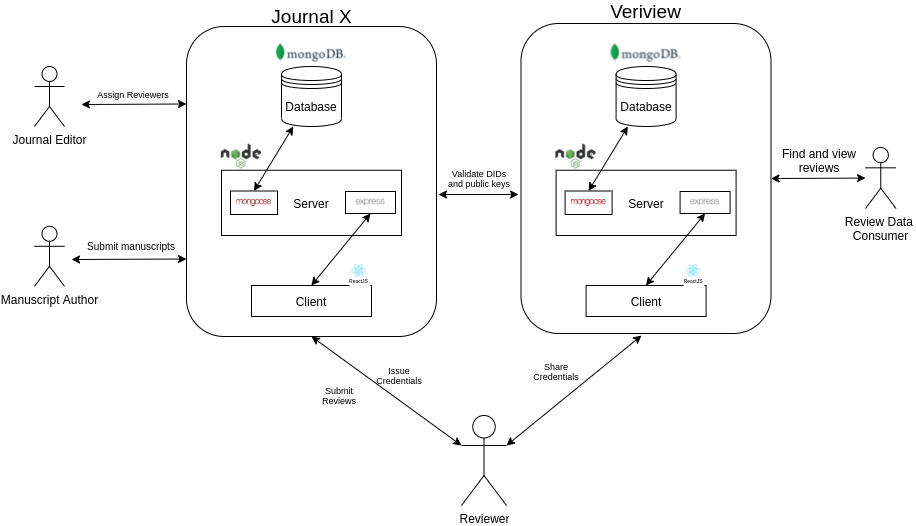
\includegraphics[width=0.8\textwidth]{figures/prototype.png}
  \caption{Overview of the architecture of the prototype} \label{fig:prototype}
\end{figure}

\subsection{Journal X}

Journal X is the simulated journal management system. Researchers can create an account and submit a manuscript to the journal. The prototype is deployed at \url{https://journalx.herokuapp.com}. The application is built on a \acrshort{MERN} stack. The MongoDB database stores the \lstinline{User} and login \lstinline{Token} data, in addition to the \lstinline{Manuscript}, \lstinline{Review}, and the \lstinline{ReviewTask} data. The \acrshort{CRUD} operations are done through the Mongoose driver that runs on the NodeJs Express server.

As the issuer identifier in the credentials \acrshort{DID}s are used. The preferred \acrshort{DID} method is \lstinline{did:web} and the \acrshort{DID} of the implemented journal is \lstinline{did:web:journalx.herokuapp.com}. The document contains the public keys belonging to the journal that are used in credential verification. The \acrshort{DID} document is given in Listing \ref{lst:did-doc}.

\lstinputlisting[language=json, caption={Journal X \acrshort{DID} document},label={lst:did-doc}]{code/did-doc.json}

In Journal X, a researcher can view their manuscripts' statuses as in Figure  \ref{fig:submit-manuscript} and submit a manuscript that they want to be published in the form page upon clicking "Submit Manuscript". 

\begin{figure}[htpb]
  \centering
  
\includegraphics[width=0.8\textwidth]{figures/submitManuscript.png}
  \caption{View and submit manuscripts} \label{fig:submit-manuscript}
\end{figure}

Upon submission, a review process has been initiated for the manuscript. The editor can assign reviewers for the manuscript and change the publication status of the manuscript according to the reviews as in Figure \ref{fig:editor}. Users can see their assigned reviews (Figure \ref{fig:reviewer-screen}) and submit the review through the form page. The review includes an optional title, the content, an optional competing interest statement and a recommendation such as "Accept", "Minor Revision", "Major Revision" or "Reject". Finally they can see their submitted reviews as in Figure \ref{fig:view-review} and download the verifiable credential by clicking "Issue Credential".

\begin{figure}[htpb]
  \centering
  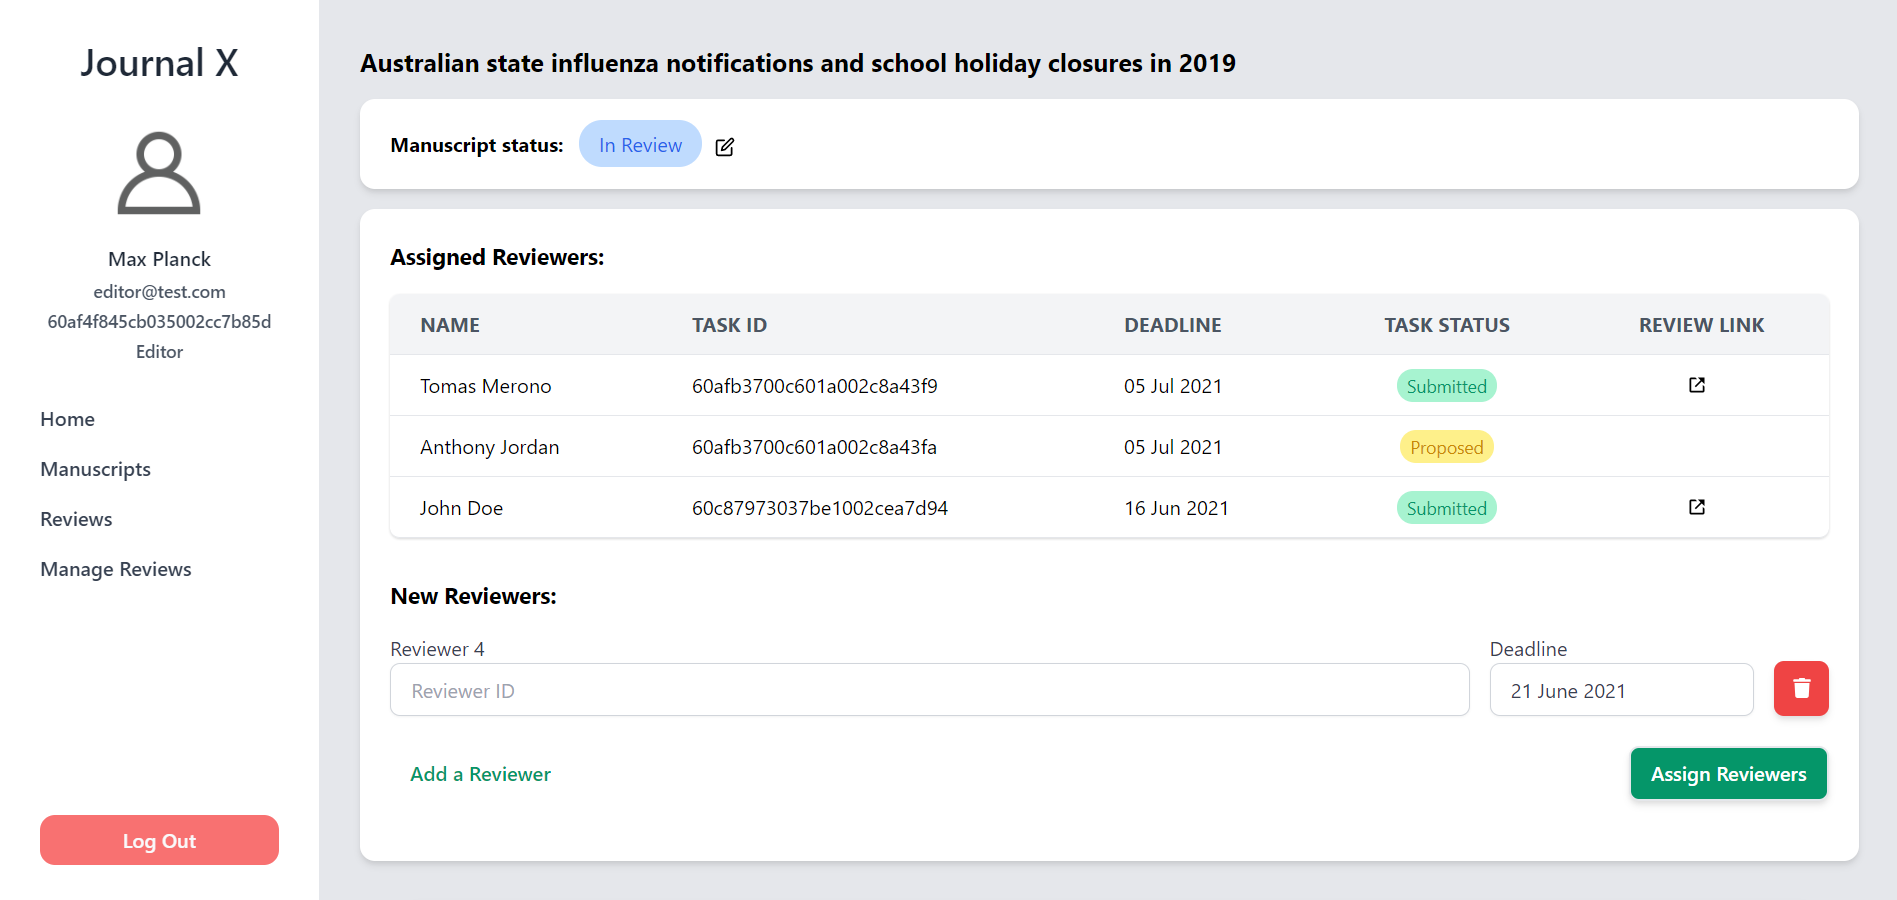
\includegraphics[width=0.8\textwidth]{figures/editor.png}
  \caption{Editor manage review process screen} \label{fig:editor}
\end{figure}

\begin{figure}[htpb]
  \centering
  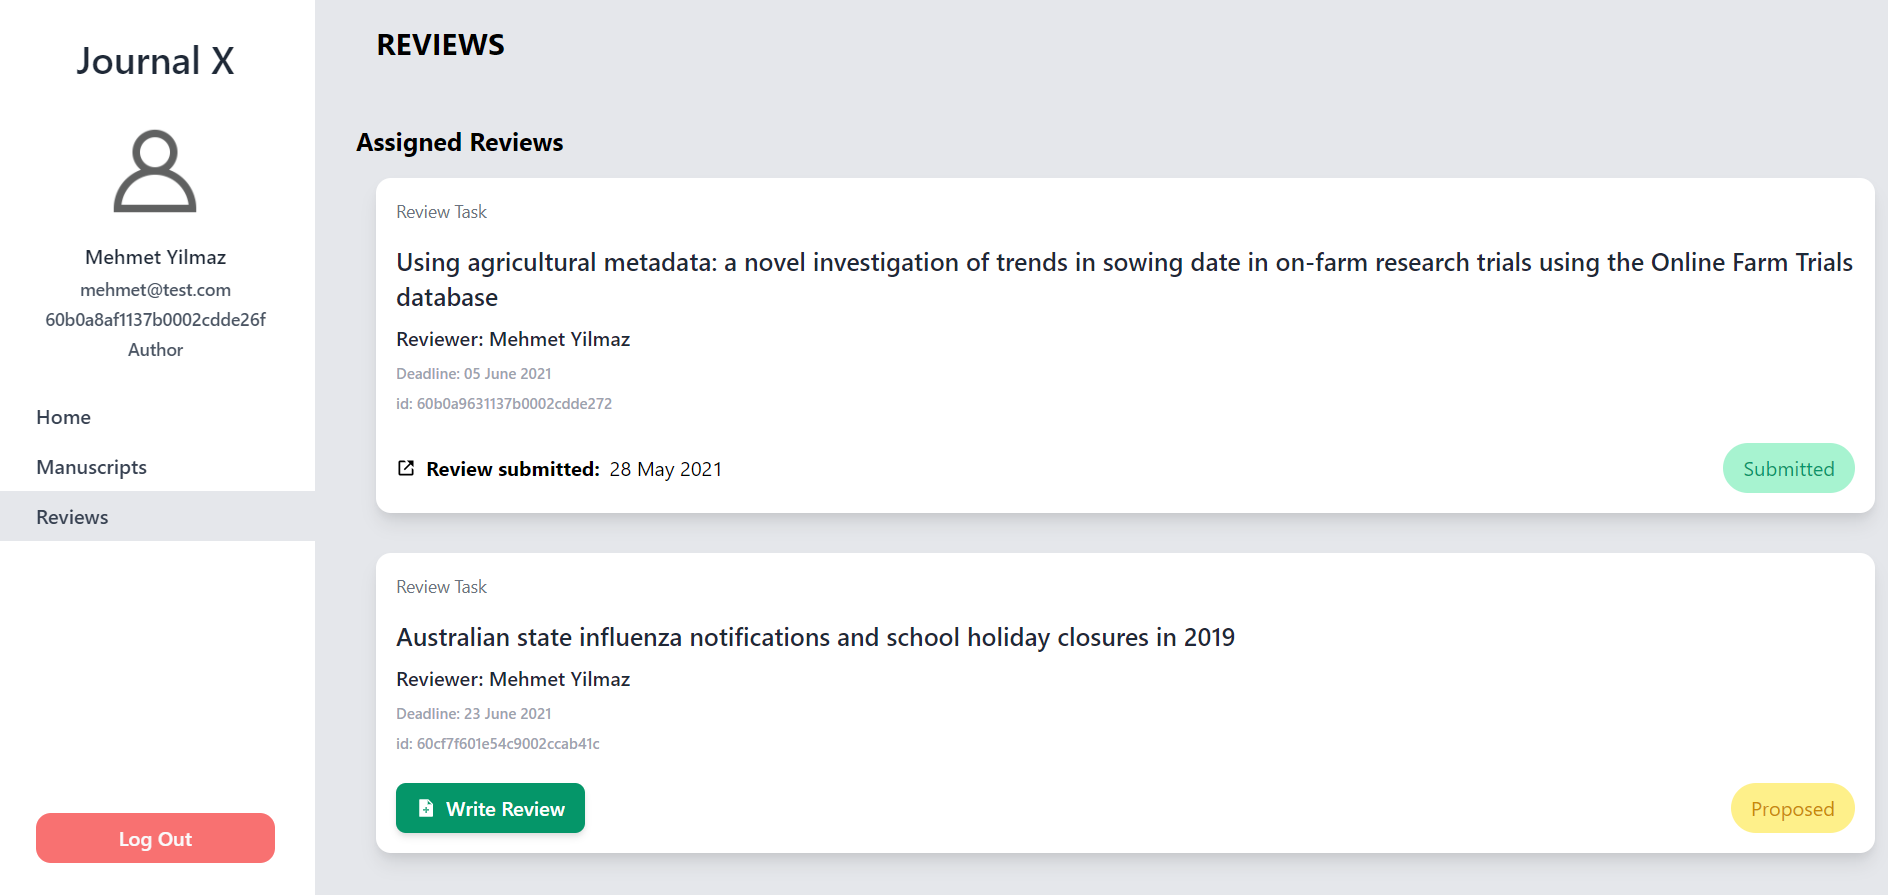
\includegraphics[width=0.8\textwidth]{figures/reviewerScreen.png}
  \caption{Reviewer dashboard} \label{fig:reviewer-screen}
\end{figure}

\begin{figure}[htpb]
  \centering
  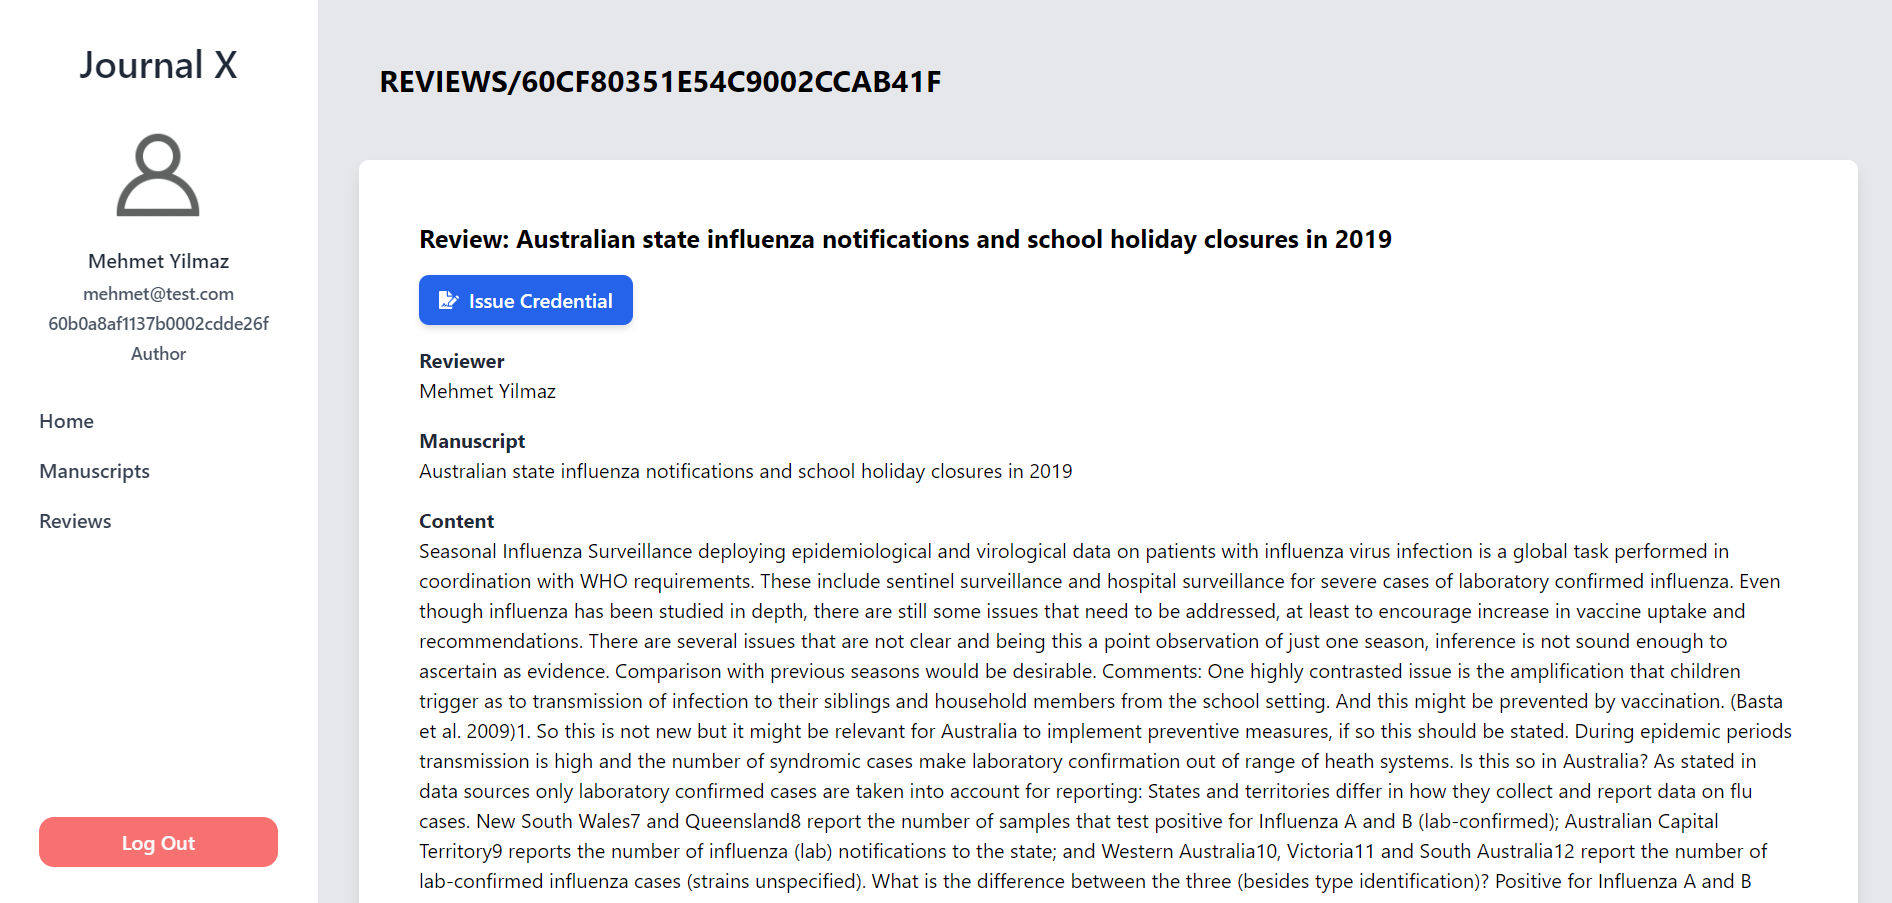
\includegraphics[width=0.8\textwidth]{figures/viewReview.png}
  \caption{View review and issue verifiable credential} \label{fig:view-review}
\end{figure}

When the credential is issued, it is downloaded to the reviewer's device as a file in \lstinline{.jsonld} format. Ideally these credentials are stored encrypted in a credential wallet or another dedicated application and only leave the application after deriving the credential. However, the prototype does not include a wallet since there are no existing ready to use wallet applications that support BBS+ signatures and credential derivation. Also, the credential exchange should be mediated by a secure protocol.  Instead, the users download their credentials plain text and use this file in the platforms. The secure connection is also out of scope of this work and only a HTTPS connection is established between the user and the platforms.

\subsection{Veriview}

Veriview is the conceived peer review showcasing platform of the prototype. Similar to Journal X, it is built on the \acrshort{MERN} stack. The working application is deployed at \url{https://veriview.herokuapp.com}. In addition to a journal account, the users need to create a Veriview account. Once they have an account, they can add the review credentials they obtained from journals to their Veriview profile. To add a peer review, the users are prompted to select the local credential file on their device. The input credential will be parsed and verified on the application. The verification at this stage is on the original credential, and the user will be able to derive a credential in the next steps. The application will first fetch the contexts (unless they are cached), and check the syntax of the document. Following, it will fetch the issuer document, which in our case is the Journal X's \acrshort{DID} document. Since it is a \lstinline{did:web} identifier, it will fetch the \acrshort{DID} document at \url{https://journalx.veriview.com/.well-known/did.json}. Next, the signature on the credential, which is under the attribute \lstinline{proof} will be validated against the public verification key of the \acrshort{DID} document. If all steps succeed, the document will be marked verified with a green check on top as in Figure \ref{fig:select-attributes}

\begin{figure}[htpb]
  \centering
  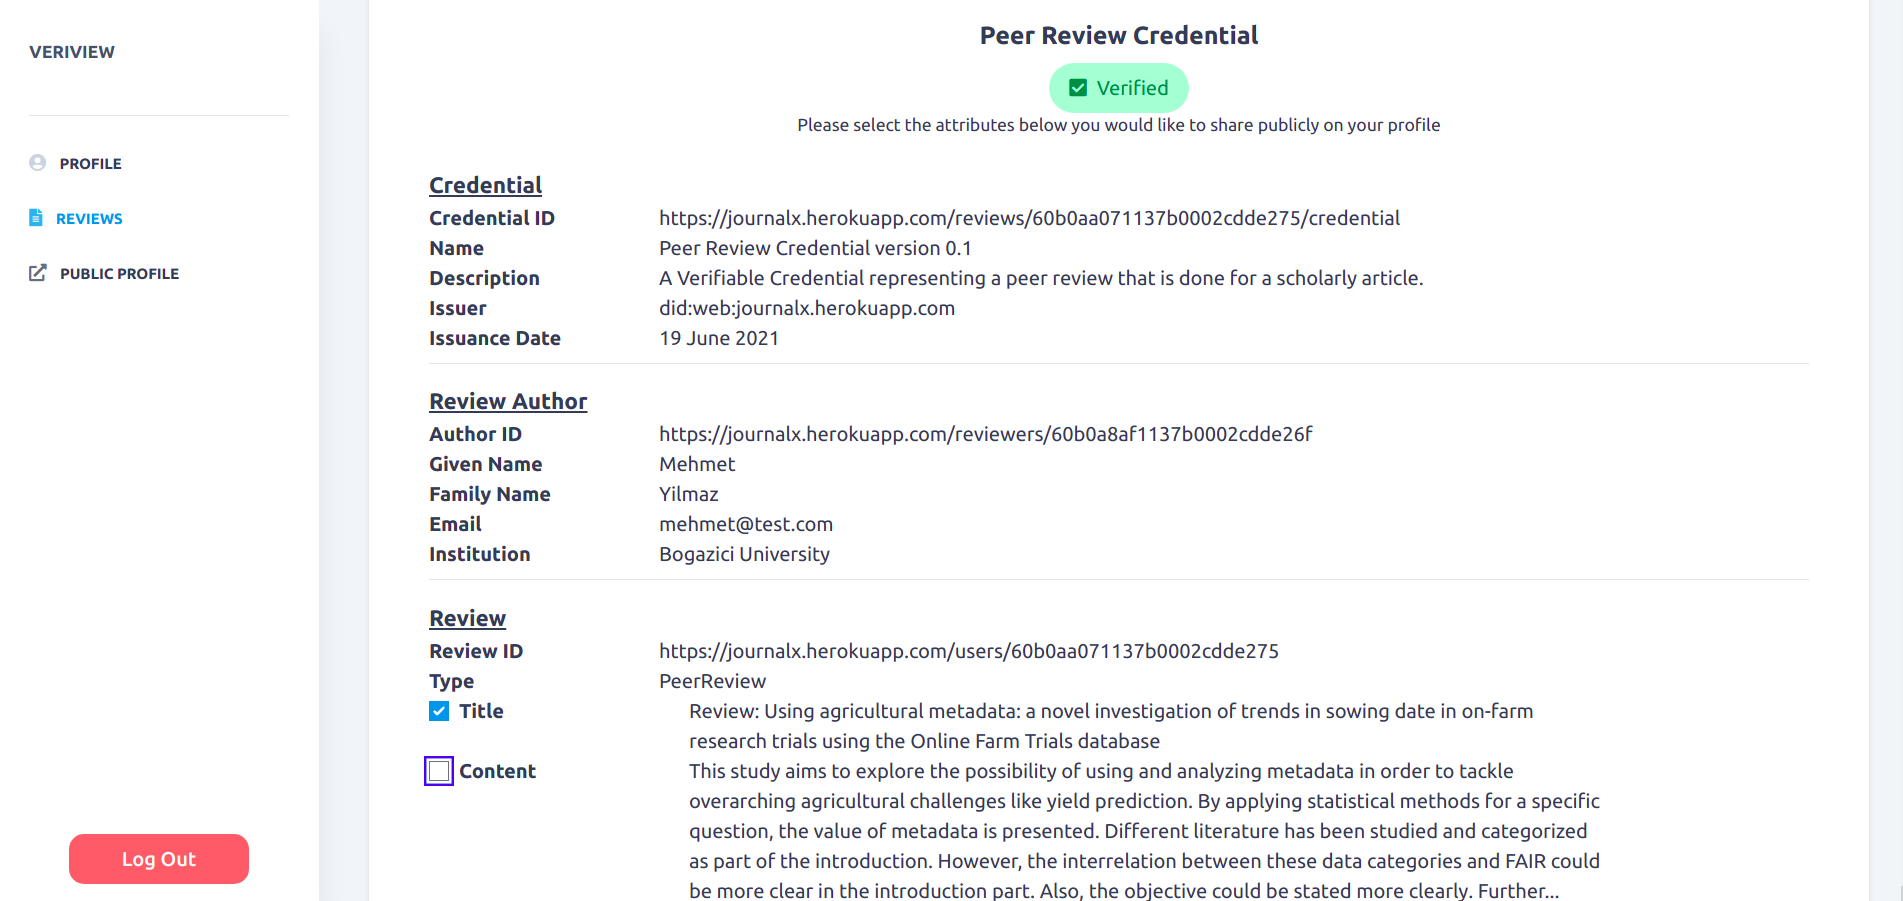
\includegraphics[width=0.8\textwidth]{figures/select-attributes.png}
  \caption{Adding the review credential to Veriview and selecting attributes} \label{fig:select-attributes}
\end{figure}

Here, the users can choose which attributes of a review they want to share publicly on their profile. For instance, typically a blinded review should not contain any information that would identify the review, meaning the review date, title, content, the manuscript title, and the manuscript abstract should be excluded. The interface does not allow users to exclude some fields such as the credential issuer, issuance date, review id, and review author information.

After selecting the attributes to be shared, a new credential will be derived from the original credential, which only contains the chosen attributes and a \lstinline{proof} attribute of type \lstinline{BbsBlsSignatureProof2020}. This proof is different than the signature of the original document, and is a zero-knowledge proof that the holder of this document knows a valid signature over the complete credential that is issued by the same issuer. The users can review the derived credential and add it to their profile by clicking "Submit". It is also possible to view the raw document in \acrshort{JSON-LD} format by clicking "Show Code", and download the derived credential (Figure \ref{fig:derived-credential}).

\begin{figure}[htpb]
  \centering
  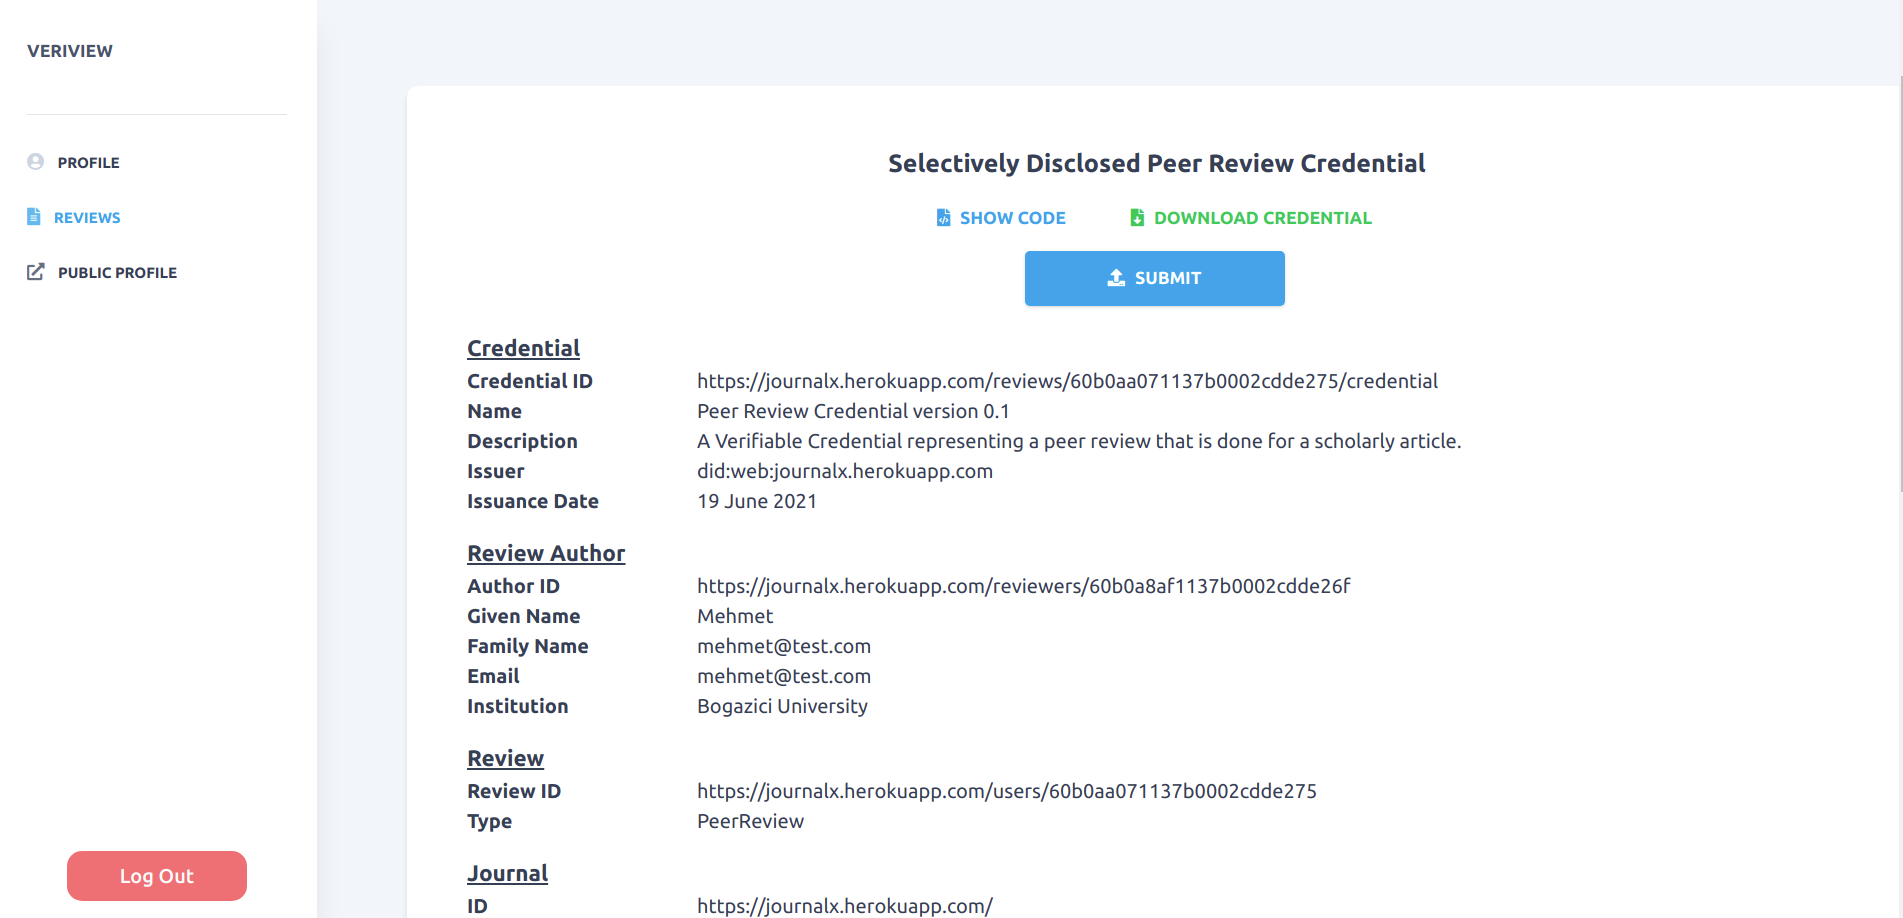
\includegraphics[width=0.8\textwidth]{figures/derived-credential.png}
  \caption{The selectively disclosed peer review credential} \label{fig:derived-credential}
\end{figure}

Finally users can view their profiles, and their profiles are publicly available at their unique \acrshort{URL}s. On this page the review consumers can view the review contributions of a researcher.

\subsubsection{Comparison to the conceptual design}

The prototype is not a complete implementation of the conceptual design and only serves the purpose of demonstrating the technical feasibility of the conceived system, in particular the \acrshort{VC} implementation of peer reviews including the issuance, verification of the credentials, and the selective disclosure with the zero-knowledge proofs. Below are the main differences between the original design and the implemented prototype.

\begin{itemize}
    \item \textbf{Wallet:} Verifiable credentials normally should be stored and managed in wallet applications as they contain personal information. Another reason is to be able to complete other actions in \acrshort{VC} exchanges such as establishing a secure channel, selective disclosure, verification of credentials or wrapping credentials into verifiable presentations. The implementation does not include a wallet application and the mentioned steps are either omitted or done by different parts of the application. As a secure channel only \acrshort{HTTP}S connection is available and users directly download the credentials issued by the journal. As discussed, usage of verifiable presentations in credential exchange can be skipped by checking the identifier/email information of the review author. Additionally the Veriview application is used for credential verification, and selective disclosure. When a user adds a credential, the client side application fetches the \lstinline{issuer} \acrshort{DID} and verifies the credential. Users can also derive selectively disclosed credentials on the client side without the credentials being sent to the server. 
    
    \item \textbf{Review Invitation:} In a typical review process, journal editors invite researchers to review manuscripts. Researchers can accept or reject this invitation. However, in the prototype the editor can directly assign researchers as reviewers.
    
    \item \textbf{Credential Issuance:} Upon receiving the peer review journals may decide not to immediately issue peer review credentials to review authors. Journals may wait until the decision to publish the manuscript has been made or until the manuscript is published. In the prototype review authors can immediately download their review credentials.
    
    \item \textbf{Duplicate Reviews:} When users are adding a review credential to their profile, it should be checked if the review has already been added to avoid showing a review contribution multiple times as if they are different reviews. This can be simply done by requiring the identifier of the review in the credential, which is unique and consistently assigned by the issuing journal. The prototype does not complete this check to allow first time users test out selective disclosure without needing to write a new review, but it is a fairly simple change.
    
    \item \textbf{Reviewer Identifier/Email Check:} As discussed in the design section, it is possible to skip some extra steps in the \acrshort{VC} verification by checking the review author identifier/email when adding a review to the Veriview. Even though users provide an email when signing in to the Veriview prototype, this check is not made as it requires an implementation of email and \acrshort{DID} verification, and it is out of the scope of the prototype.
    
\end{itemize}
